\documentclass{article}
\usepackage{graphicx}
\usepackage[margin=1.5cm]{geometry}
\usepackage{amsmath}

\begin{document}
\twocolumn

\title{Thursday Warm Up, Unit 1: Filter Design}
\author{Prof. Jordan C. Hanson}
\maketitle

\section{Memory Bank}

\begin{enumerate}
\item \textbf{The convolution theorem} states that the Fourier transform of the convolution of two functions is the same as the product of the Fourier transforms of the two functions.
\item \textbf{Recursive filter formula}.  Start with convolution, and let $h[i] = a_i$.  The result is
\begin{equation}
y[n] = \sum_{i=0}^N a_i x[n-i]
\end{equation}
Now add \textit{feedback from prior output samples} to compute the \textit{next} output sample, using coefficients labeled $b_i$.  Note that $b_0 = 0$, as this corresponds to $y[n]$.
\begin{equation}
y[n] = \sum_{i=0}^N a_i x[n-i] + \sum_{i=1}^N b_i y[n-i] \label{eq:1}
\end{equation}
\end{enumerate}

\section{FFT Convolution}

\begin{enumerate}
\item Write a short \verb+octave+ script that convoles a \textit{gaussian pulse} with a square pulse.  A gaussian pulse is a sine wave with a gaussian envelope.  This calculation arises in certain branches of quantum mechanics. Sketch the output below: \\ \vspace{4cm}
\end{enumerate}

\section{LP and HP Recursive Filters}

\begin{enumerate}
\item Suppose we want to implement a \textbf{low-pass} recursive filter (Fig. \ref{fig:1}).  (a) If our sampling rate $f_{\rm s}$ is 10 kHz, and we need a cutoff frequency $f_{\rm C}$ of 1 kHz, what is the ratio of these?  This is the unitless cutoff frequency. (b) Find $x = \exp(-2\pi f_{\rm C})$, using the unitless cutoff frequency. (c) Calculate $a_0 = 1-x$, and $b_1 = x$, with all other $a_i$ and $b_i$ set to zero. (d) Simplify Eq. \ref{eq:1} to account for the constraints on $a_i$ and $b_i$.  (e) Implement this in an \verb+octave+ script, and find the step response.
\item Repeat the previous exercise, but for a \textbf{high-pass} recursive filter (Fig. \ref{fig:2}), using $a_0 = (1+x)/2$, $a_1 = -(1+x)/2$, and $b_1 = x$. Use the same unitless cutoff frequency.
\end{enumerate}

\begin{figure}[hb]
\centering
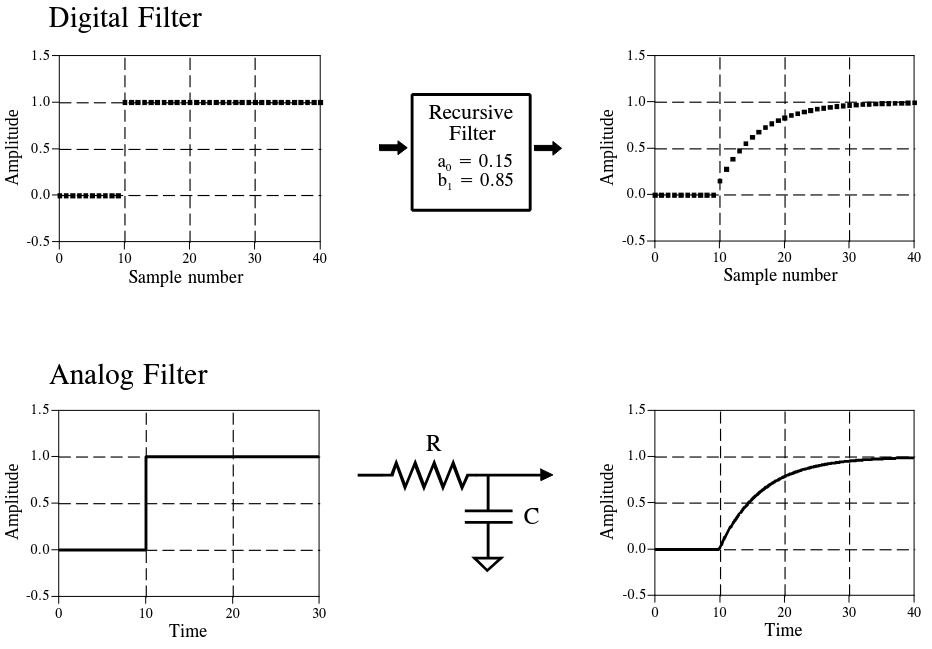
\includegraphics[width=0.5\textwidth]{lp_rec.png}
\caption{\label{fig:1} A low-pass RC-like recursive filter.}
\end{figure}
\vspace{1cm}
\begin{figure}[hb]
\centering
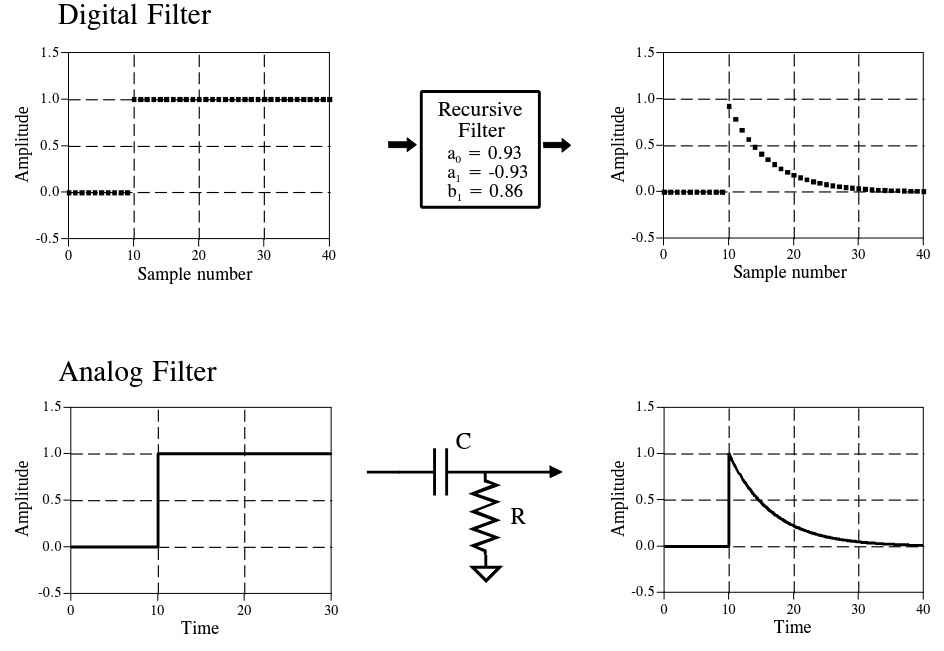
\includegraphics[width=0.5\textwidth]{hp_rec.png}
\caption{\label{fig:2} A high-pass RC-like recursive filter.}
\end{figure}

\end{document}
